\section{The Descent of the Absolute}

In \emph{Man and his Becoming}, \textbf{Rene Guenon} describes the manifestation of the Self into the human state according to the Vedanta. The West has its own Traditional understanding. It is not different, but it is worth the trouble to redo the same project in more Western terms. This post can be the barest outline, and specific topics will be developed in future posts.

By the Absolute, we mean generally what is called Brahman, that is, whatever is beyond being. The Self (Atma) is the principle of the individual. As such, the Self is beyond all manifestation and time. The descent through the degrees of being begins with formless manifestation, then to formal manifestation in the subtle state and ultimately to the gross state. This is not a process that occurs in time. Nor does the Self descend through these stages, since it is their principle.

\begin{wrapfigure}{rt}{.35\textwidth}
 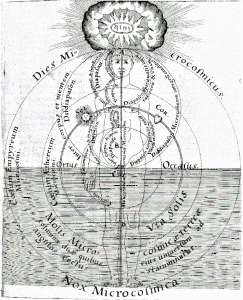
\includegraphics[scale=.5]{a20210307TheDescentoftheAbsolute-img001.png} 
\end{wrapfigure}

A difficult notion to accept is that “time”, as we know it, is a feature of the human state. Once understood, however, many fruitless philosophical and theological conundrums are resolved.

The human state is said to be “rare”, in the sense that it is just one possible state out of many. The situation of the being in the human state allows the being to act in a way to acquire knowledge, unlike other states that are passive. Thus, it is special and should not be squandered.

These are the primary degrees although each one can be further divided, potentially indefinitively, into subdegrees. The Self becomes conscious of the world of sensible manifestation through:

\begin{itemize}
\item Thought 
\item Inward senses or wits 
\item Individual consciousness 
\item Five senses 
\item Five organs of action 
\item Life force 
\end{itemize}
\subsection*{Buddhi}
The buddhi, Universal Spirit, or Higher Intellect belongs to the realm of formless manifestation. As such it is the first degree of the manifestation of the Self. The possibilities of manifestation become ideas or essences in the Higher Intellect.

It is the principle of the formal manifestation of the Self and thus is the unifying principle. Rene Guenon calls it the “Spiritual Sun which shines at the center of the entire being.” Put another way, it is the “spark of divinity,” even if only virtually.

Thought is the faculty which gives form to ideas and associates them to each other; thought is how we experience the Higher Intellect.

However, in the Higher Intellect, it is not yet individual consciousness.

\subsection*{Manas}
The characteristics of the Manas, or Universal Soul, relate to faculties of the formal order.

Mental faculty or inward sense. Individual thought, memory, imagination

\begin{itemize}
\item\textbf{Five elements}: Ether, air, fire, water, earth
\item\textbf{Five Senses}: sight, hearing, smell, taste, touch
\item\textbf{Five Wits}: memory, estimation, fantasy, imagination, and common sense
\item\textbf{Five actions}: Ingestion, excretion, reproduction, locomotion, grasping
\end{itemize}

From the esoteric perspective, the senses are prior in the ontological sense. Moderns believe that somehow matter is creating sensations in the brain. The same for the other features. The desire for locomotion and grasping, for example, direct evolution. They are not the serendipitous results of a random evolutionary process.

Also, the ideas of the elements determine gross manifestation, not the other way around.

\subsection*{Causal Body}
The causal body is the dividing line between pure Being and the individual being. As such, it is the essence of the human being, that is, what he is born with. Boris Mouravieff explains it as analogous to the unfolding of a movie film:

\begin{quotex}
Each human being, then, is born with his own particular film [destiny]. This represents the field of action in which man is called to apply his conscious efforts. 

\end{quotex}
The causal body is still in the formless order. Rene Guenon describes it as

\begin{quotex}
the totality of the possibilities of manifestation which Atma comprises within itself, in its permanent actuality in the principial and undifferentiated state. [It] enjoys the plenitude of its own being, and it is in no way really distinct from the ‘Self’; it is superior to conditioned existence, which presupposes it, and it is situated at the level of pure Being. 

\end{quotex}
But when viewed in relation to formal manifestation,

\begin{quotex}
it can be said to represent principial or causal form, that by which form will be manifested and actualized in the succeeding stages. 

\end{quotex}
Hence, it is the

\begin{quotex}
principle and cause of all manifestation and the source from which manifestation is developed in the multiplicity of its different states and more particularly, as concerns the human being, in its subtle and gross states. 

\end{quotex}
The principles and causes are described below.

\paragraph{Non-dual awareness}
At the level of Being, the causal state is non-dual awareness, beyond the subject-object distinction. As such it creates the sensible world through the three forces:

\begin{enumerate}
\item \textbf{Active force}: The idea or essential cause. This makes the world intelligible. 
\item \textbf{Passive force}: Matter or substantial cause. Matter is the principle of multiplicity. It is pure quantity without any qualities. 
\item \textbf{Neutralizing force}: Consciousness. 
\end{enumerate}
When the horizontal substantial cause meets the vertical essential cause, the thing arises. Yet it is not real unless and until there is consciousness. In the causal state, the virtual senses of the manas are actualized so that the world of the senses — or corporeal world — arises.

Yet there is no separation between subject and object, Self and the world. The self is said to participate in the world because there is no distinction.

\paragraph{Categories}
The categories of being are the most general of all genera and determine the essence of the human being at birth. One's essence is unalterable. The tendency today is to regard these categories as arbitrary, inessential, and even unjust. However, they make the being unique and distinct from other beings. Aristotle's categories are helpful to understand this. Here are some examples.

\textbf{Substance}: Obviously, in this case, the substance is to be a human being.

\textbf{Time and place}: The human being is born at a particular time and place.

\textbf{Qualities}: The human being is born with certain qualities. These include the following, although it is unnecessary to specify precise details, which the reader can easily do.

\begin{itemize}
\item Habits and Dispositions 
\item Natural Capabilities and Incapabilities 
\item Affective Qualities and Affections 
\item Shape 
\end{itemize}
\textbf{Relations}: this includes all the relationships that the being is born into. Among them are parents, family, nation, race, religion, and so on.

\textbf{Sex}: Sex is not a substance because both male and females are fully human, and not different species of the genus “human”. Nor does sex fit into a category of being, as the difference is above a category. Nevertheless, sex is not conventional, nor simply biological. Nevertheless, sex is “constitutive for the person” not an “attribute of the person”.

\paragraph{Messengers of Gods}
In the Divine Comedy, Dante describes the ascent through the planetary spheres and the hierarchy of angels. In the descent of the being, the angels and celestial objects play a role in the progressive manifestation of the being.

The angels mediate the stages of manifestation. In a moral world, there needs to be an adversary, which makes evil a possibility of manifestation. Hence, there are fallen angels that distort the process.

\paragraph{Macrocosm}
The Microcosm is the Macrocosm is a truism in Hermetism. This must, however, be understood in its interiority, not as material forces and objects. This is the true astrology: the Spheres of Heaven correspond to aspects of our soul. Thus, there is the Moon of the being, Venus of the being, and so on. The effects of Mercury, Venus, Mars, Jupiter, and Saturn, understood in their interiority, on our lives need not belabored here.

\paragraph{Archetypes}
Besides the archetypes which manifest from above, there are also

\begin{quotex}
the archetypes which manifest themselves endlessly in history and in each individual biography — they are mythological symbols pertaining to the domain of time. (Valentin Tomberg) 

\end{quotex}
For examples, the prophets can be understood that way: there is the Adam of the being, Noah of the being, Abraham of the being, and so on. Here only Adam concerns us, for the others are part of the re-ascent.

Adam is the father of all humankind. Due to that, we are born in a condition of ignorance, malice, concupiscence. This separates the human microcosm from the purity of the macrocosm. These conditions are not part of the being's essence, because they can be altered and overcome in life. Hence, any attribute or quality that is sinful cannot be an essential part of the human being.

\subsection*{Ego}
Thinking separates the nondual awareness of the causal state into subject and object. At this stage individuality is realized. Thought creates the idea of the Ego experiencing objects “out there, right now”. So Rene Descartes’ quip, “I think, therefore I am,” is exact, presuming that it refers to the Ego of the human state, not the Real Self. The Ego in the individual state forgets its true identity.

\subsection*{Subtle Body}
The human being manifests as a subtle body and a gross, or physical, body. These correspond respectively to two of the conditions of manifestation: psyche (or life) and matter. So in addition to the features of the human being acquired from the vertical direction, he is also subject to the psychical and material currents active in the time and place of his birth.

The subtle body is further subdivided in three: the intellectual, animal (or emotional), and vegetable souls. The soul divisions are porous, so there are no hard divisions between them. Features of each can appear in the others. That is why animals can display intelligence or why a human can feel pleasure in intellectual attainment. More often, the mixture is deleterious. Mouravieff makes that clear:

\begin{quotex}
In fact, we have neither a pure thought nor a pure feeling: nor are our actions pure. Everything in us is mixed and even entangled, often by all sorts of considerations which either come from the intellectual centre, tarnishing the purity of our feelings by its calculations, or from the emotional centre, which clouds the calculations of the intellectual centre. 

\end{quotex}
Since this topic has been covered numerous times, we just need a cursory mention here. A full explanation would require a book.

\begin{itemize}
\item\textbf{Mental Body:}
Intellectual soul Activities related to thinking. The lower part includes opinons and discursive thinking. The higher part is intuitive thinking.

\item\textbf{Astral Body:}
The Sensitive soul or animal soul is the center of the lower mental functions, emotions, feelings as well as refined sensations and passions;

\item\textbf{Etheric body:}
Also known as vegetable soul or life body. This is the center of the faculties of action and sensation, which relate to the corresponding features of the Manas.
\end{itemize}

It also directs unconscious processes like nutrition, growth, secretion, and reproduction.

The motor centre governs instinctive life as well as movement and all mental activity: its action is thus distributed throughout the physical body.

\subsection*{Gross Body}
Matter is not productive of anything. It is only alive when animated by the etheric body. When that latter separates from the gross body, the body dies and decays.

Even the gross body has levels: first, it is subject to the laws of physics, then those of chemistry, and finally biology.

Nevertheless, The qualities of the human being are determined ontologically prior to biological processes. Hence, biology does not create the human being, but rather the other way around.

Nevertheless, the gross body is the medium through which one's destiny is played out. The physical world is the unconscious of the Self.

\subsection*{Level of Being}
A fundamental principle is that what is ontologically prior comes after in time. Hence, at the level of the gross body, it appears that life (etheric body) follows matter, then consciousness, and eventually thought. In the temporal sense, the world appears to “evolve” from the lower to the higher.

However, ontologically there is no absolute standard of time, so the states are, from the viewpoint of the Self, simultaneous. Where the Self “is” in the states of the being is determined by where the Self is focusing consciousness.

\subsection*{Sources}

\textsc{Barfield, Owen}: \emph{Saving the Appearances}

\textsc{Dante}: \emph{Divine Comedy}

\textsc{Guenon, Rene}: \emph{Man and his Becoming according to the Vedanta}

\textsc{Lewis, C. S.}: \emph{The Discarded Image}

\textsc{Shankara}: \emph{Tattva Bodhah}, Commentary by Swami Tejomayananda

\textsc{Shankara}: \emph{Vivekacudama\d ni}, Commentary by Swami Dayananda Saraswati

\textsc{Mouravieff, Boris}: \emph{Gnosis}

\textsc{Aristotle}: \emph{Categories}

\flrightit{Posted on 2021-03-07 by Cologero}